\documentclass[letterpaper,11pt]{article}
\usepackage{graphicx}
\usepackage{listings}
\usepackage{hyperref}
\usepackage{amsmath}
\usepackage{url}
\def\UrlBreaks{\do\/\do-}
\usepackage[normalem]{ulem}
\newcommand{\tab}[1]{\hspace{.2\textwidth}\rlap{#1}}
\usepackage{xcolor}
\usepackage{sectsty}
\sectionfont{\color{blue}}
\usepackage{titlesec}
\usepackage{fancyvrb}
\usepackage{listings}
\usepackage{caption}
\usepackage[vertfit]{breakurl}
\sloppy
\usepackage{fancyvrb}

\titleformat{\section}
{\color{blue}\normalfont\Large\bfseries}
{\color{blue}\thesection}{1em}{}

\lstset{
        basicstyle=\footnotesize,
        breaklines=true,
}

\begin{document}
\begin{titlepage}
\begin{center}
\Huge{Assignment 9}
\\
\Large{CS595}
\\
\Large{Introduction to Web Science}
\\
\Large{Old Dominion University}
\\
\Large{Computer Science}
\\
\Large{Due: 11:59 pm Dec 04}
\\
\Large{Lulwah Alkwai}
\\
\end{center}
\end{titlepage}
\newpage

\section*{}
(10 points; 2 points for each question and 2 points for aesthetics)

Support your answer:
include all relevant discussion, assumptions, examples, etc.

\section*{Question 1}
1.  Create a blog-term matrix.  Start by grabbing 100 blogs; include:\\
http://f-measure.blogspot.com/\\
http://ws-dl.blogspot.com/\\
and grab 98 more as per the method shown in class.

Use the blog title as the identifier for each blog (and row of the matrix).  Use the terms from every item/title (RSS) or entry/title
(Atom) for the columns of the matrix.  The values are the frequency of occurrence.  Essentially you are replicating the format of the"blogdata.txt" file included with the PCI book code.  Limit the number of terms to the most "popular" (i.e., frequent) 500 terms,
this is *after* the criteria on p. 32 (slide 7) has been satisfied.
\newpage
\subsection*{Answer One-}
To solve this question I have done the following steps:
\begin{itemize}
  \item I grabbed 100 blogs, I started out with the two required blogs and then added some other blogs from my office friends and went from there and grabbed more using the method mentioned in class.The result was blogdata1.txt.
  
  \item For the second step which is creating a matrix I used the code generatefeedvector.py and made the  required adjustments.

The matrix required was using blog title as the identifier for each blog row and using the terms for the columns of the matrix;the values are the frequency of occurrence.

The adjustment that were made were that the TFIDF is calculated as the score that balances the frequency of a term in a document vs. frequency of a term in all the documents.Also limit the number of terms to the most "popular" 500 terms.

note:to run the code I had to download the feedparser using the command:
\begin{lstlisting}[frame=single]
pip install feedparser
\end{lstlisting}

\end{itemize}
\newpage
\section*{Question 2}
2.  Create an ASCII and JPEG dendrogram that clusters (i.e., HAC) the most similar blogs (see slides 12 and 13).  Include the JPEG in your report and upload the ascii file to github (it will be too unwieldy for inclusion in the report).
\newpage
\subsection*{Answer Two-}
I used the code clusters.py. However some files needed to be downloaded on my computer such as PIL. To do so I had to install clang, so I downloaded the command line tools from Xcode. Then I had to download the PIL file from \url{http://www.pythonware.com/products/pil/}.
Finally I used the following commands:
\begin{lstlisting}[frame=single]
brew install libjpeg
pip install PIL
\end{lstlisting}

The resulting graph is shown at figure 1. The closest blog to f-measure was the week-end.And the closest blog to the ws-dl blog is the orcale blog.

\begin{figure}[!ht]
\centering
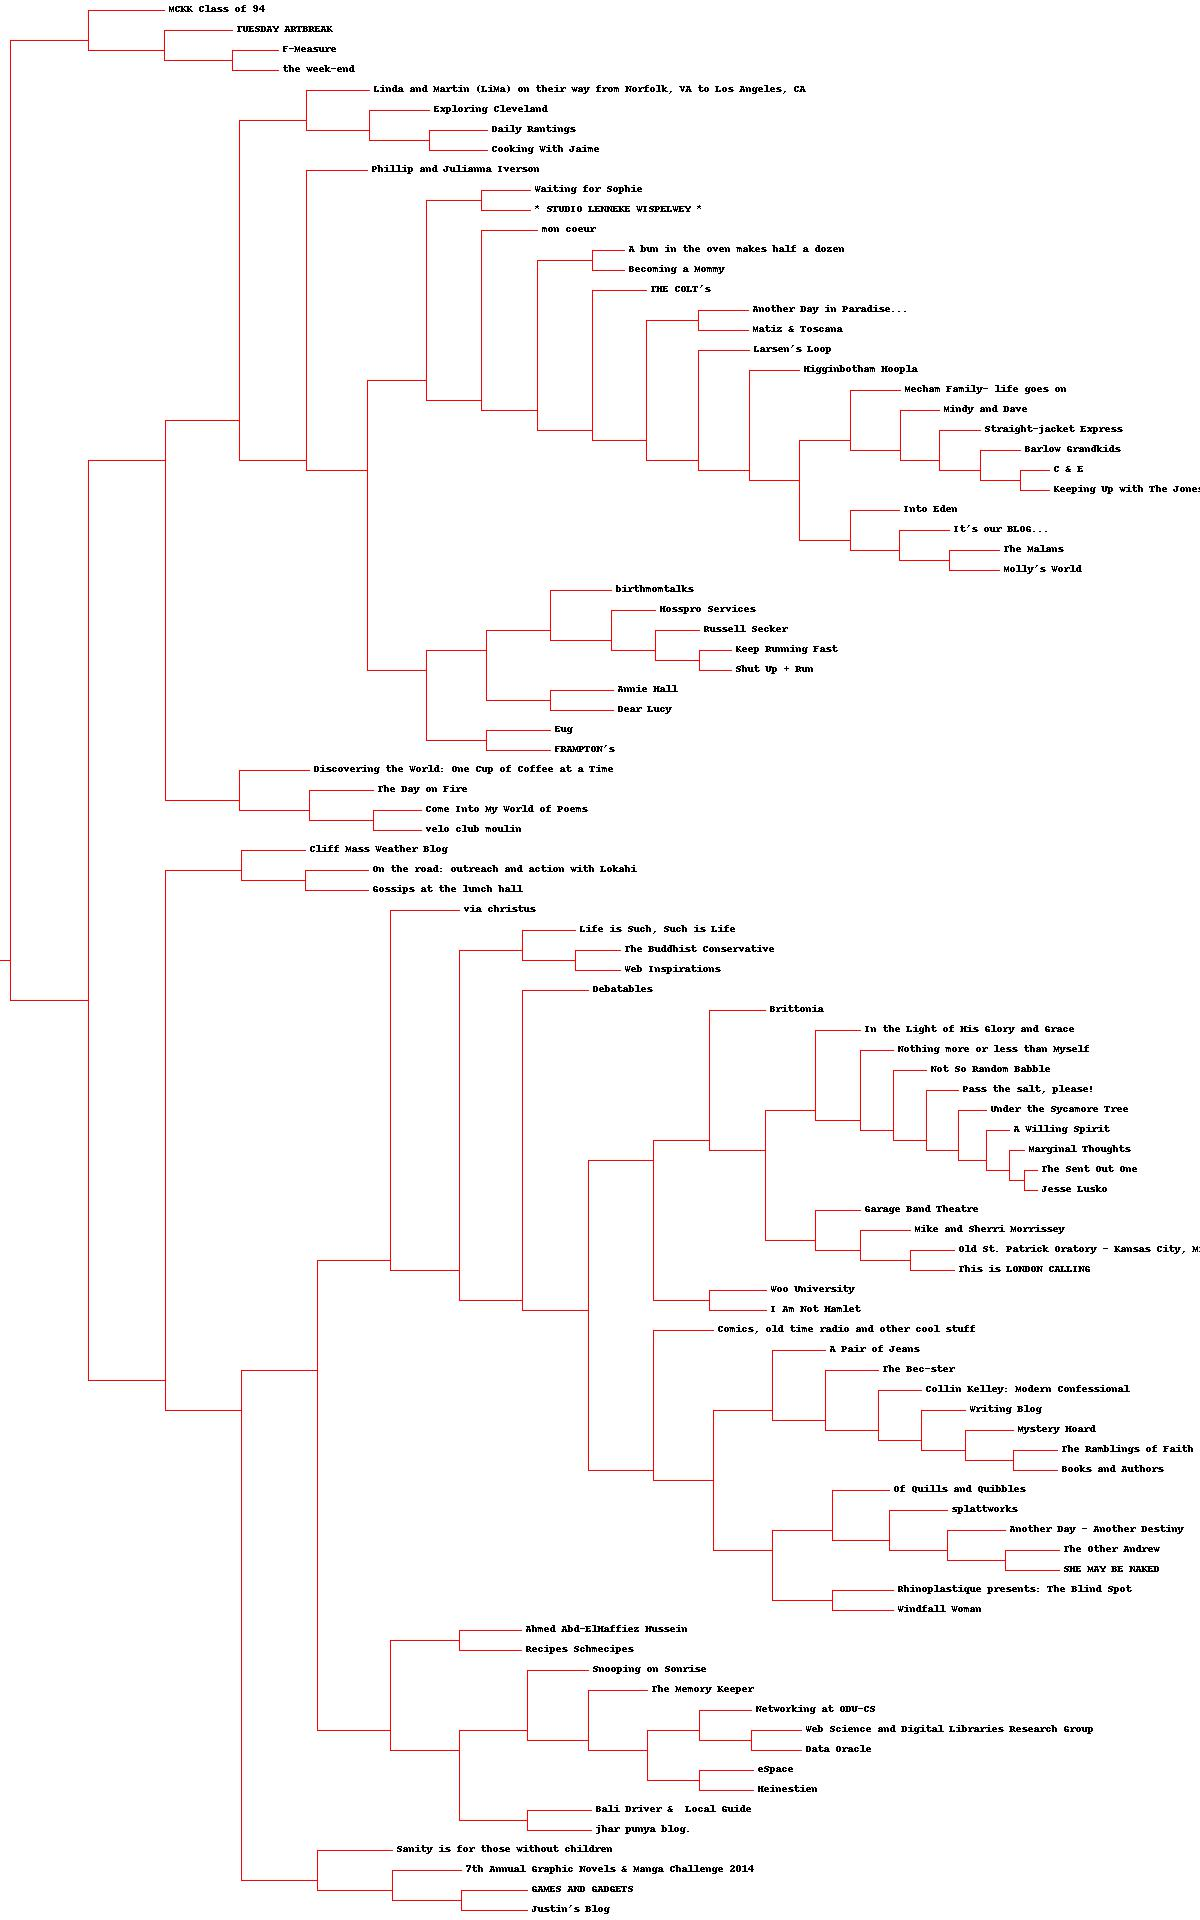
\includegraphics[width=0.8\textwidth]{blogclust.jpg}
\caption{blog clustuer}
\label{fig:blog clustuer}
\end{figure}

\newpage
\section*{Question 3}
3.  Cluster the blogs using K-Means, using k=5,10,20. (see slide 18).
How many interations were required for each value of k?
\newpage
\subsection*{Answer Three-}
Again using the code clusters.py I added the K-Means.The iterations were as following:
\begin{lstlisting}[frame=single]
K=5
Iteration 0
Iteration 1
Iteration 2
Iteration 3
Iteration 4
Iteration 5
Iteration 6

K=10
Iteration 0
Iteration 1
Iteration 2
Iteration 3
Iteration 4
Iteration 5
Iteration 6
Iteration 7
Iteration 8

K=20
Iteration 0
Iteration 1
Iteration 2
Iteration 3
\end{lstlisting}

So for K=5 there was 7 iterations, for K=10 there were 9 iterations and for K=20 there are 4 iterations.

\newpage
\section*{Question 4}
4.  Use MDS to create a JPEG of the blogs similar to slide 29. How many iterations were required?
\newpage
\subsection*{Answer Four-}
Again using the code clusters.py I added the MDS to create a JPEG of the blogs.The code used was from the class slides. The number of iteration is 419. As seen in the OutputData.txt. The resulting graph is figure 2.

\begin{figure}[!ht]
\centering
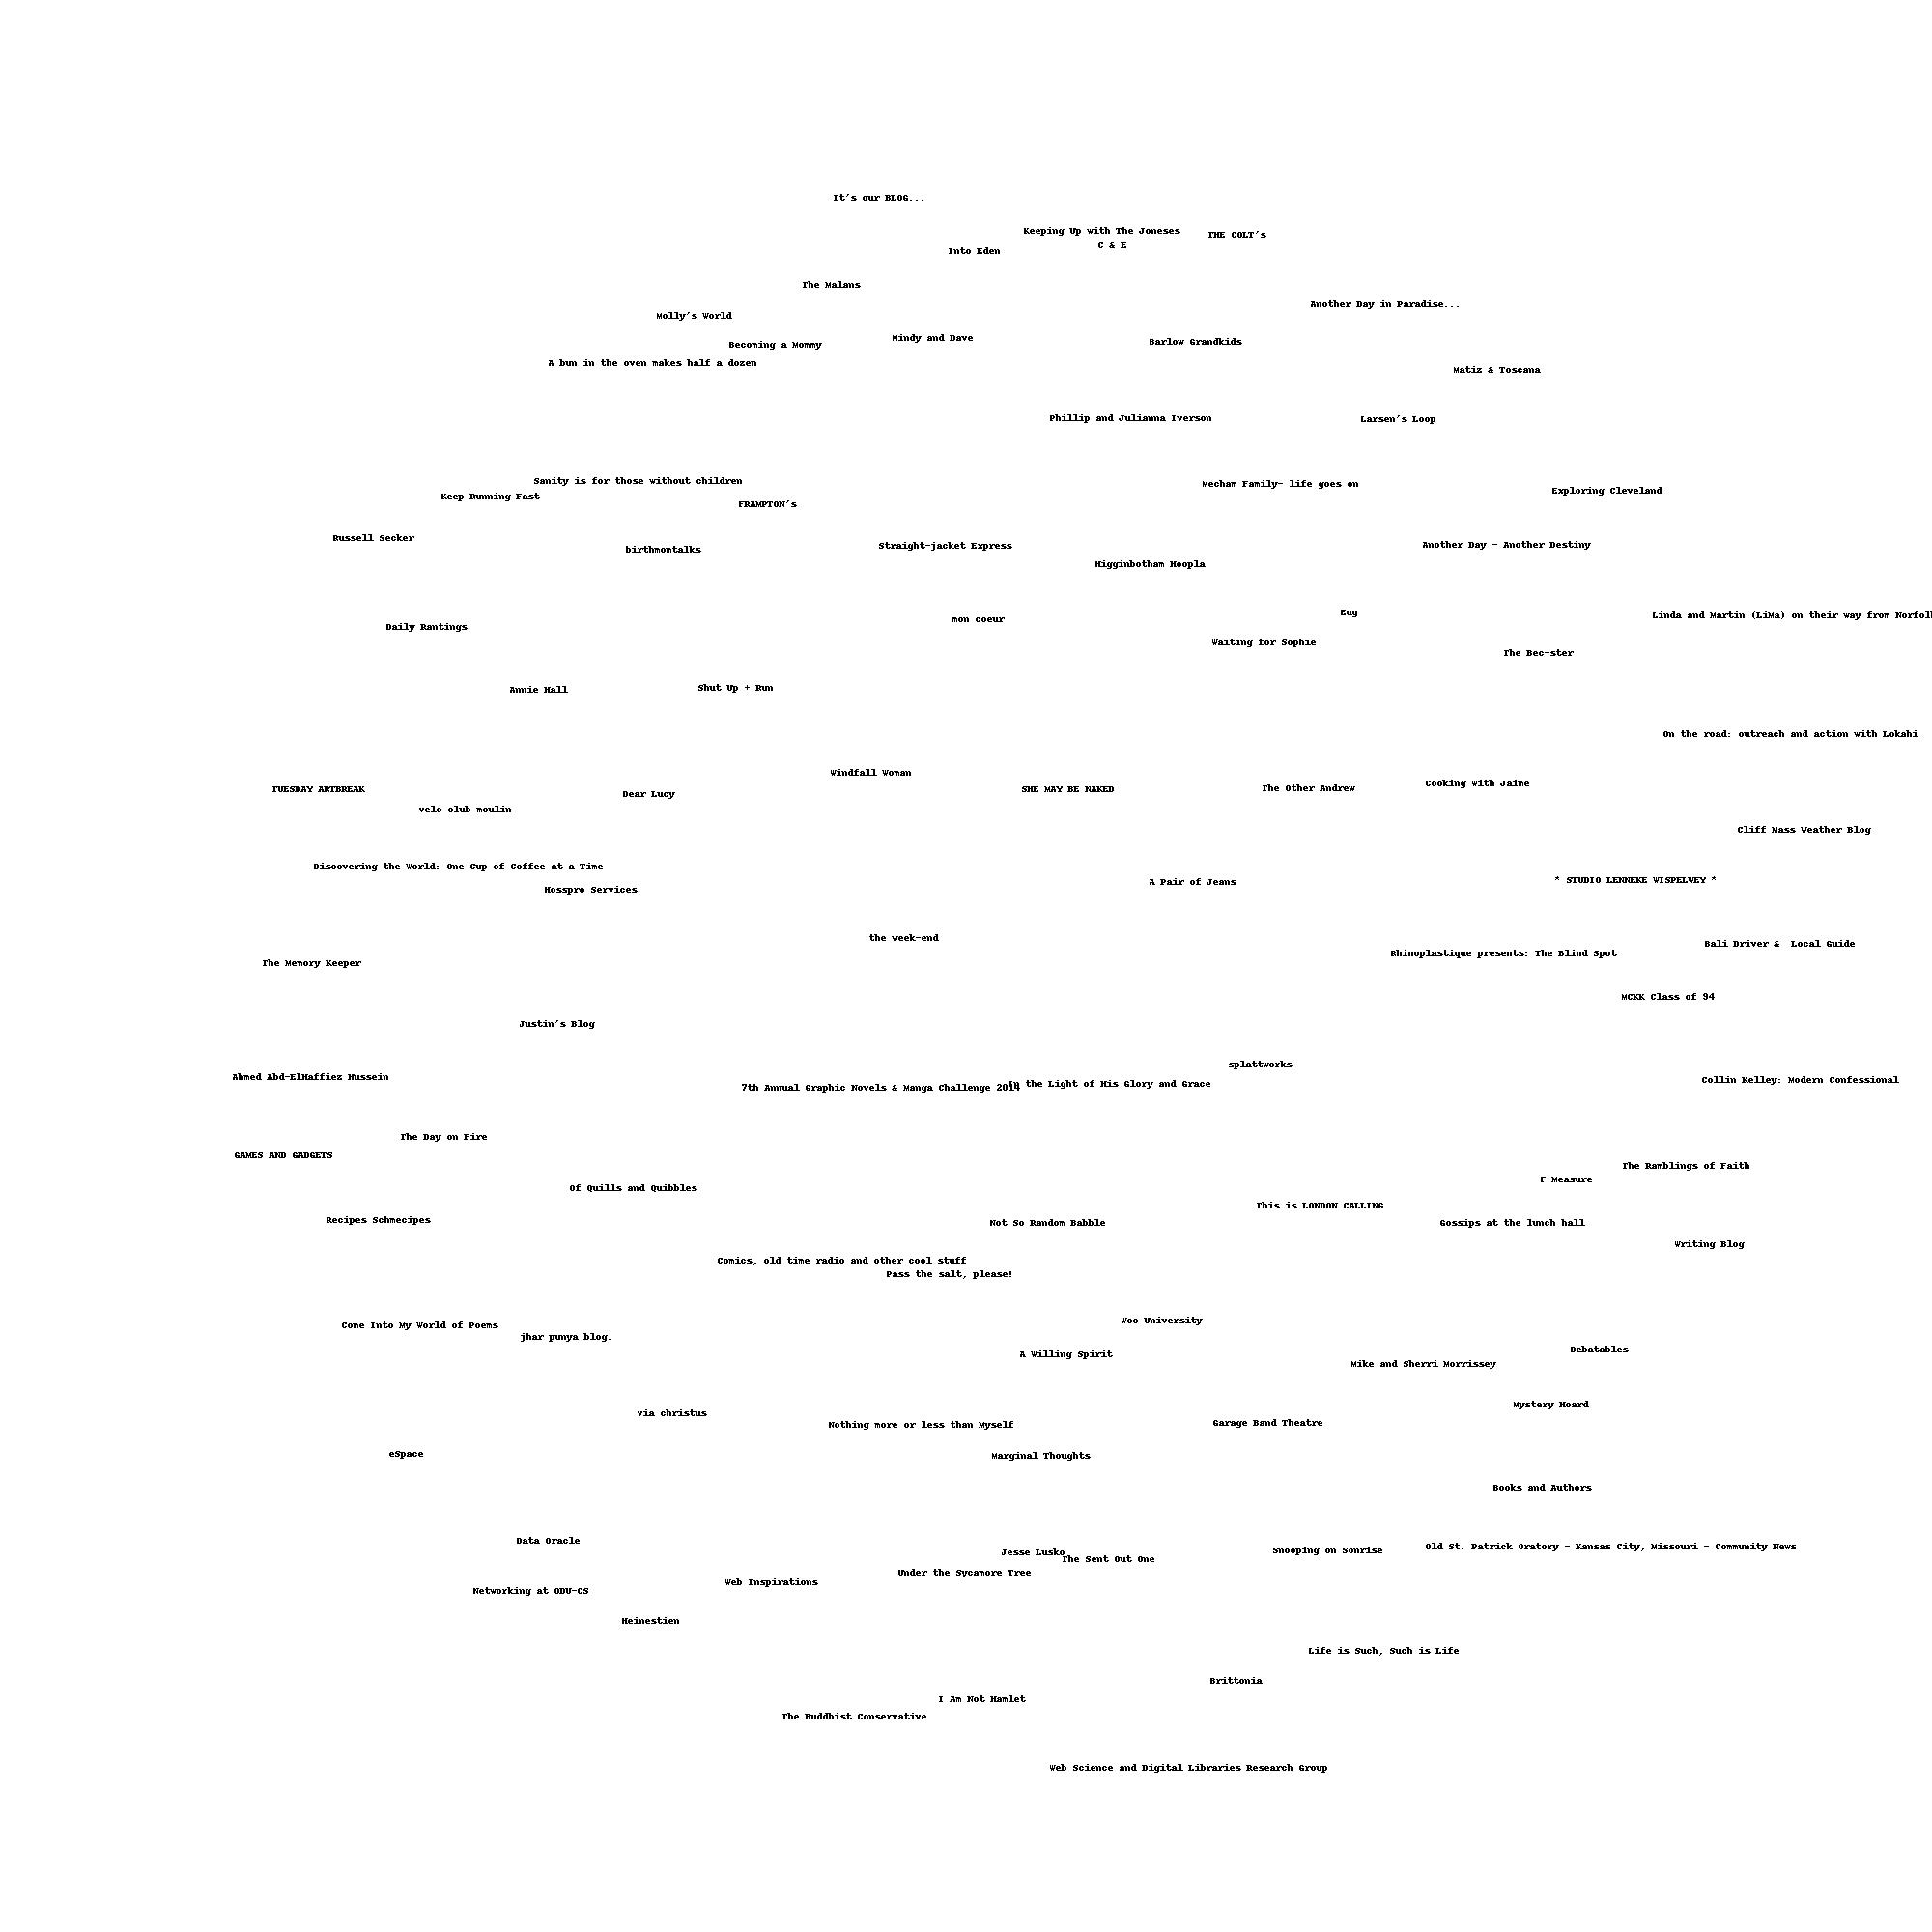
\includegraphics[width=0.8\textwidth]{blogs2d.jpg}
\caption{MDS to create a JPEG }
\label{fig:MDS to create a JPEG }
\end{figure}

\newpage
\section*{Question 5}
==========================================
The questions below is for 5 points extra credit
==========================================

5.  Re-run question 2, but this time with proper TFIDF calculations instead of the hack discussed on slide 7 (p. 32).  Use the same 500 words, but this time replace their frequency count with TFIDF scores as computed in assignment 3.  Document the code, techniques, methods, etc. used to generate these TFIDF values.  Upload the new data file to github.

Compare and contrast the resulting dendrogram with the dendrogram from question 2.

Note: ideally you would not reuse the same 500 terms and instead come up with TFIDF scores for all the terms and then choose the top 500 from that list, but I'm trying to limit the amount of work necessary.
\newpage
\subsection*{Answer Five-}
No attempt.
\end{document}